% !TEX root = C:\Users\Jan\Documents\dev\Risk-Measurement-Framework\masterthesis_tex\masterthesis_main.tex
\section{Implementation}
\label{sec:implementation}

Afer explaining and discussing the concept this section describe the implementation of the technical framework RMF by following the procedures of ISO 27004 \cite{ISO_27004_2009}. The technical RMF uses Python 3.7 \cite{10.5555/1593511} as the programming language and ART as the basis. Beside the attacks given by the ART, there is a function from the technical RMF to execute individual attacks. This technical RMF should be used a step ahead of using the framework of Schwerdtner et al. \cite{DBLP:journals/corr/abs-2011-04328}.

\subsection{Structure of the RMF}

\subsubsection*{Directory tree}

The RMF is structured as follows: \\

\dirtree{%
.1 rmf/.
.2 attacks/.
.3 art/.
.4 backdoors.py.
.2 backdoors/.
.3 png-Files.
.2 measurement/.
.3 monitoring.py.
.3 log.py.
.3 measurement.py.
.2 visualizations/.
.3 data\_output.py.
.3 plot.py.
.2 log\_file.log.
.2 case\_study.py.
}

\hfill \break \noindent The \textit{png-Files} are used by the \textit{backdoors.py} script to add patterns into the images that are the backdoor triggers. Both folders \textit{measurement} and \textit{metrics} contain implementations to monitor the collected data for the risk measurement and evaluate it. The \textit{visualizations} folder shows the measurement results and summarize them into one output file.

\subsection{Implementing the risk indicatiors}

The risk indicators are the main part for the risk measurement. Therefore the risk indicators are used through the complete risk measurement. Every risk indicator is implemented as an own
function in the RMF. This makes it possible to measure the risk indicator values at every step during the ML model training. The goal is to use measure the risk indicator values with the
original training data and the manipulated training data. The $accuracy=\frac{n(correctly\_predicted)}{n(all)}$ is implemented as Nguyen and Zeigermann \cite{9783960101925} describe it.
The next risk indicator is the attack time which checks the time an attack needs to be executed and if the attack is executed during training or inference time. Depending on the targeted phase, the function for this risk indicator checks the ML for vulnerabilites. Every Vulnerability increases a counter to check how much exploits are in the ML algorithm. Since in this thesis only backdoor attacks are performed, finding vulnerabilities refers to checking if backdoor triggers are in images \cite{DBLP:journals/corr/abs-1708-06733}, \cite{DBLP:journals/corr/abs-1907-07296}. This matching of patterns in images do the Fast Library for Approximate Nearest Neighbors (FLANN) \cite{DBLP:journals/corr/FuC16} in relation with the Scale Invariant Feature Transform (SIFT) algorithm \cite{Songtao2017AnIM}. The following Python algorithm shows how both work in combination: \\

\begin{lstlisting}
  img1 = cv.imread('box.png',cv.IMREAD_GRAYSCALE)          # queryImage
  img2 = cv.imread('box_in_scene.png',cv.IMREAD_GRAYSCALE) # trainImage

  # Initiate SIFT detector
  sift = cv.SIFT_create()

  # find the keypoints and descriptors with SIFT
  kp1, des1 = sift.detectAndCompute(img1,None)
  kp2, des2 = sift.detectAndCompute(img2,None)

  # FLANN parameters
  FLANN_INDEX_KDTREE = 1
  index_params = dict(algorithm = FLANN_INDEX_KDTREE, trees = 5)
  search_params = dict(checks=50)   # or pass empty dictionary
  flann = cv.FlannBasedMatcher(index_params,search_params)
  matches = flann.knnMatch(des1,des2,k=2)
\end{lstlisting}

\textit{img1} is the pattern that the algorithm should find in \textit{img2}. SIFT is feature extraction algorithm which detects points of an image's scale space. That detection comes from a variable-scale Gaussian convolution that takes an input image. The next part is the positioning of feature points, then the algorithm assigns the direction of these feature points with a pixel gradient histogram. The last part of the algorithm is a description of each feature point's uniqueness by a feature vector. After SIFT the FLANN algorithm searches based on Approximate Nearest Neighbor (ANN) search \cite{DBLP:journals/pami/MujaL14} with a KD-Tree \cite{DBLP:journals/cacm/Bentley75}. After each match the RMF uses the prediction function of Keras to check if the poisoned image predicts the correct target label and then saves the correct label and expected target label as a key-value pair to count how many images are missclassified correctly. This label relation should evaluate in more detail the extent of the attack on the ML model. \\
Attack specificity is an risk indicator that measures if the attack is targeted or untargeted. The ART attacks have a parameter that takes a target optionally. If the target is random, then there is no specific label. If it is targeted, there is a specific label where a certain number of images in percentage are poisoned or specific images of a targeted label. As next is the TP, TN, FP, FN. Keras show these values with a
implemented function in this technical framework. The computational resources get the values from the operating system for the specific executed Python script. The attacker's knowledge is
implemented based on the attack. For example, if the \textit{Pattern Backdoor Attack} is implemented in the ML model, then the function for the attacker's knowledge returns the steps to
implement this specific attack \cite{bsi_2013}. Attacker's goal \cite{DBLP:journals/corr/abs-2012-04884} can be an inference failure, obtain secret information, or executing a denial-of-
service. The goal of this risk indicator is to evaluate it based on monitored data of the attack. The attack must have characteristics that represent the goal an attacker has. An
inference failure happens during the testing phase. So when an attacker try to execute an inference failure he could use exploratory attacks \cite{tabassi2019taxonomy} or evasion attacks \cite{DBLP:conf/sp/Carlini017}. Obtain secret information can be for example stealing model attacks \cite{DBLP:journals/corr/abs-2105-00623}, \cite{DBLP:journals/wicomm/ZhangLGQTZ20}. Denial-of-service attacks have the goal to slow
down the ML model or crash the ML model completly \cite{DBLP:journals/sensors/VaccariAC20}. If one of these goals is identified then this function returns pre-determined steps on how to achieve this goal. If an attacker tries to missclassify the ML model based on backdoor attacks, then the goal could be an inference failure because the image classification fails during inference time. To achieve this goal the attacker has to develop a backdoor attack. The difference between achieving this goal and getting the knowledge of the attacker is about how they develop the backdoor attack to get what he wants and how much he knows to implement the attack into the ML model. The goal do not concentrate on specific attacks, only on what the attacker have to do in general. \\
Subsection \ref{sec:impl_backdoor_attacks} explains how the attacks in the measurement methods are implemented and what an attacker have to do to implement them into a ML model. After that, subsection \ref{sec:impl_threat_model} explains how to get the risk indicator values if an attack is executed.

\subsection{Implementing backdoor attacks from the ART}
\label{sec:impl_backdoor_attacks}

The following three attacks are all based on the ART \cite{art2018} and represent white-box and black-box attacks and both targeted and untargeted attacks. These attacks are the main factor to assign the values to the base measures. The attacks already differentiate between the original and poisoned dataset for evaluation. To implement the attacks and measure the attacker's goal to get an inference failure, the following steps has an attacker to do \cite{DBLP:journals/corr/abs-2003-03675}: \\

\begin{enumerate}
  \item Taking one or more backdoor pattern
  \item Taking target labels corresponding to the patterns
  \item Place it at a specific or random location
  \item Place the backdoor trigger to a subset of the original data
  \item Mix it with the original data
  \item Mapping the backdoor triggers to the corresponding target labels
\end{enumerate}

\subsubsection*{Backdoor attacks from the ART}
\label{sec:backdoors_art}

All backdoor attacks use the \textit{Pattern Backdoor Attack} \cite{DBLP:journals/corr/abs-1708-06733} class which expects a pattern argument. The pattern is a picture which is for the poisoned images in the training data. The pattern must be implemented before training and choose a random selection of images. This is implemented in the RMF as follows:

\begin{lstlisting}
  n_train = np.shape(x)[0]
  num_selection = num_of_rand_images
  random_selection = np.random.choice(n_train, num_selection)
  x = x[random_selection]
  y = y[random_selection]
\end{lstlisting}

Then the arguments $x$ and $y$ are passed to the poisoning function from the ART. $x$ and $y$ are parameters which the function expects when calling it. Appendix \ref{sec:frame_func}
describe the functions and parameters. Further it is important that the shape of the images from the training data are \textit{N, H, W, C} or \textit{N, C, H, W}. $N$ is the number of
images in the batch, $H$ is the image height, $W$ is the image width, and $C$ is the channel number of an image such as grayscale or RGB. After adding a backdoor as a pattern to the
random images, the poisoned images are replaced back to the training data. These poisoned images are saved in a different folder to check if the images are missclassified after or while
testing the ML model.\\


The first attack uses the \textit{Pattern Backdoor Attack} class without any other backdoor classes from the ART. This attack which bases on Gu et al. \cite{DBLP:journals/corr/abs-1708-06733} is a black-box attack which is untargeted. In the RMF it uses a pattern backdoor which Figure \ref{fig:original_example} and Figure \ref{fig:poisoned_example} show as the
difference between the original and the poisoned image. The goal of this attack is to change the original label to a random other label. This attack can be executed without any
information because it is not important which training data the ML model use and what ML model is used for the training itself.

\begin{figure}[!tbp]
  \centering
  \begin{minipage}[b]{0.4\textwidth}
    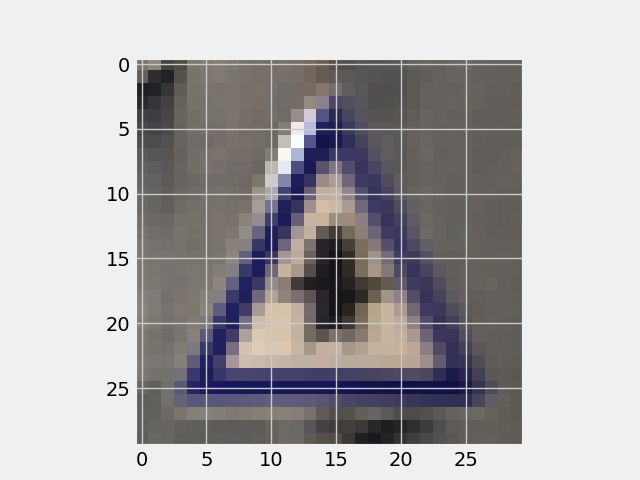
\includegraphics[width=8cm]{pictures/original_example.png}
    \caption{Street sign without a backdoor pattern with the label \textit{Right-of-way at intersection}.}
    \label{fig:original_example}
  \end{minipage}
  \hfill
  \begin{minipage}[b]{0.4\textwidth}
    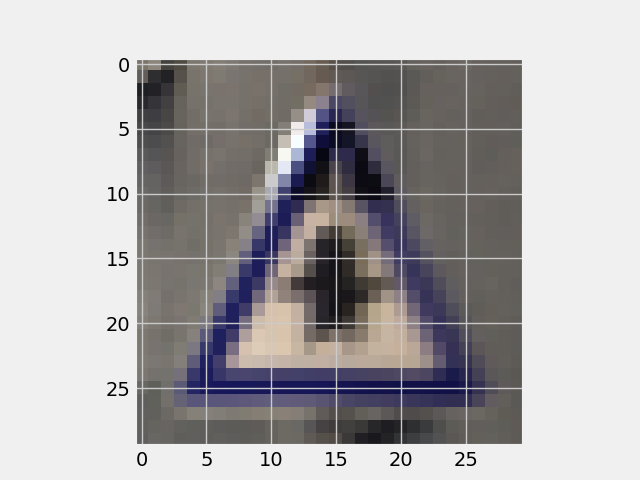
\includegraphics[width=8cm]{pictures/poisoned_example.png}
    \caption{Street sign with a backdoor pattern but still with the original label \textit{Right-of-way at intersection}.}
    \label{fig:poisoned_example}
  \end{minipage}
\end{figure}

After poisoning the images these image need be copied back into the original training data. Before this can be done the poisoned data must replace the original training data which contain
no backdoor. When the RMF take the random original images, it save them into a temporary variable and then delete the images from the original training data. The next step is the
poisoning while the poisoned data and the original training data need the same shape and dimension which make it possible to copy the poisoned images. As mentioned before the poisoning
function takes four specific shapes which make it easy to have the same shape in the original training data and poisoned data. The implementation of the attack additionally shows the
effort an attacker have to implement this attack. Thus the steps can be used for the attacker's knowledge risk indicator. The steps to execute this attack are the following: \\

\begin{enumerate}
  \item Choose a backdoor pattern
  \item Take number of random images to poison
  \item Add the backdoor pattern to the images
  \item Mix poisoned images back to the original dataset
\end{enumerate}

The \textit{Clean Label Backdoor Attack} \cite{turner2018clean} poison images and misclassify during the training time. To use this attack the \textit{Pattern Backdoor Attack} must be
used before and then the clean label attack can be executed after training. After adding the backdoor trigger with \textit{Pattern Backdoor Attack} the original training data are trained
with a proxy classifier which should do the same classification tasks as the original classifier. The first poison step is selecting target images. As next the PGD (which is untargeted)
must be implemented to make it harder classify correctly. The last step is adding the backdoor trigger and add the target label. The steps to execute this attack are the following: \\

\begin{enumerate}
  \item Choose a backdoor pattern
  \item Select a source image
  \item Select a target image
  \item Reverse engineer the classifier
  \item Select a learning rate
  \item Select the number of maximum iterations
  \item Select the number (\%) of images to poison
  \item Poison the original training dataset
  \item Train the original dataset with the proxy classifier
  \item Train the poisoned dataset with the original classifier
\end{enumerate}

The \textit{Hidden Trigger Backdoor Attack} \cite{DBLP:journals/corr/abs-1910-00033} need to be executed after training. To add the backdoor, the \textit{Pattern Backdoor Attack} must be
used before. After training, the poisoned data and a smaller number of clean training inputs are used to finetune the model. Finetuning means, adjusting parameters of the ML model to
improve it with a small amount of training data to improve the performance \cite{DBLP:conf/acl/LiWTTTPBCA20}, \cite{DBLP:journals/corr/abs-2112-08691}. For the attack the poisoned data
are used with a small amount of clean training data. The following Python code shows the finetuning of a ML model where the attack is implemented.

\begin{lstlisting}
  dataset_size = size
  num_labels = label_size
  num_per_label = dataset_size/num_labels

  poison_dataset_inds = []

  for i in range(num_labels):
      label_inds = np.where(np.argmax(y_train, axis=1) == i)[0]
      num_select = int(num_per_label)
      if np.argmax(target) == i:
          num_select = int(num_select - min(num_per_label, len(poison_data)))
          poison_dataset_inds.append(poison_indices)

      if num_select != 0:
          poison_dataset_inds.append(np.random.choice(label_inds, num_select, replace=False))

  poison_dataset_inds = np.concatenate(poison_dataset_inds)

  poison_x = np.copy(x_train)
  poison_x[poison_indices] = poison_data
  poison_x = poison_x[poison_dataset_inds]

  poison_y = np.copy(y_train)[poison_dataset_inds]
\end{lstlisting}

The parameters of the \textit{Hidden Trigger Backdoor Attack} are analog to the \textit{Clean Label Backdoor Attack} but the pattern is different as the backdoor trigger which Figure \ref{fig:poisoned_hidden_trigger} shows.

\begin{figure}[ht!]
  \centering
  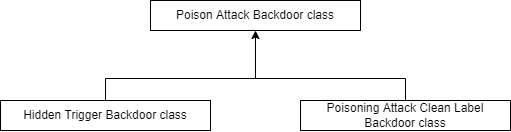
\includegraphics[width=9cm]{pictures/attack_relationship.png}
  \caption{Both attack classes (\textit{Clean Label Backdoor Attack} and \textit{Hidden Trigger Backdoor Attack}) get the backdoor from the \textit{Pattern Backdoor Attack}.}
  \label{fig:attack_relationship}
\end{figure}

The steps to execute this attack are the following: \\

\begin{enumerate}
  \item Choose a backdoor pattern
  \item Select a source image
  \item Select a target image
  \item Add the backdoor to the images
  \item Finetune the ML model with the poisoned dataset
  \item Select original training images for the finetuning
  \item Mix the poisoned with the original images
\end{enumerate}

\subsection{Implementing the threat model}
\label{sec:impl_threat_model}

The measurement methods are implemented based on the threat model of Doynikova et al. \cite{DBLP:conf/crisis/DoynikovaNGK20}. This thesis concentrates on specific risk indicators whereby the threat model functions do not expect risk indicators as arguments. The low- and high-level attributes do not need an own function because both can be saved into a list of values. So, there is only the mapping function which takes these values as arguments.

\subsubsection*{Mapping between the attributes}

The attack time and specificity are the only risk indicators which have to be mapped to the attacker's knowledge and goal. Based on the low-level attributes, the high-level attributes are additionally adjusted after the measurement. After the execution of the attacks, the values of the attack itself - specificlly the attack time - is used to measure the time an attacker needed to execute its attack \cite{DBLP:journals/corr/abs-2012-04884}. This measurement is based on the difference between training of the ML model without and with the attack. The attack time for measuring the extent of damage is used to see which vulnerabilities a ML model has during the training or test time \cite{DBLP:journals/csur/RosenbergSER21}. Because values are measured that can be used to measure the effort of an attacker, this risk indicator must be mapped. \\
For the attack specificity the RMF measures how much images are poisoned and what the attacker has to do to poison targeted images \cite{DBLP:conf/iccv/ZhuNXWW21} or how he poison random images \cite{DBLP:journals/corr/abs-1708-06733}. The amount the attack has to do to poison images is mapped into the attacker's goal and knowledge. \\
The following subsection describe how the results from the measurement methods are evaluated in the measurement construct.

\subsection{The implemented measurement construct}

After assigning the risk indicators based on the threat model of Doynikova et al. \cite{DBLP:conf/crisis/DoynikovaNGK20}, this subsection explains the implemented measurement construct starting from the base measures up to the decision criteria. \\
The measurement function is a single function which takes the base measures that has to be combined to the derived measures. To access these base measures, they must first be separated from the base measures that are given directly to the analytical model function. Figure \ref{fig:impl_meas_func} visualizes the procedure of the measurement function. The first measurement function calculates the derived measures of the TP, TN, FP, FN into the ML metrics such as F1-Score, precision-recall, and confusion matrix with the mathematical functions from Nguyen and Zeigermann \cite{9783960101925}. These ML metrics show the total results of the ML model's performance and represent as total results how the attacked changed their values.
Since the value of the $Risk$ should represent a higher risk at a high value than at a low value, the base measures as well as derived measures must output corresponding results. In order to ensure this representation, it is important for the accuracy, F1-Score, precision-recall, and confusion matrix that their reduced values due to the attack are used as a high value for the risk. Since the accuracy and the other ML metrics are represented as percentages and thus lie between $0$ and $100\%$ or $0$ and $1$, the RMF reverses these values. If the accuracy
is for example $0.06$ or $6\%$, the RMF converts this value to $9.94$ out of $10$. This allows the value to appropriately reflect how much the accuracy increases the overall $Risk$. To calculate the derived measure for the extent of damage the last value calculate how much labels are missclassified. This matching is implemented by key-value pairs whereby the key is the original predicted image and the value is the poisoned predicted image. If the poisoned prediction is the correct missclassified target label then a counter increases. Then the result of this matching can be compared with the possible number of poisoned images to check how much images are actually poisoned. The resulting percentage reflects how effective the attack was on the tested ML model. \\
In order not to depend on the different ML libraries the RMF gets its own functions of the different ML metrics. That increases the support of different Python libraries for ML risk measurement. The next function in Figure \ref{fig:impl_meas_func} combines the attack steps by adding all steps together.

\begin{figure}[ht!]
  \centering
  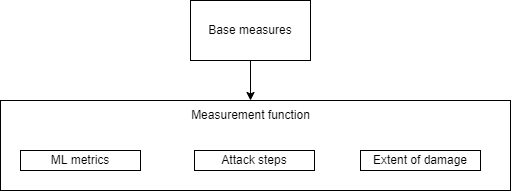
\includegraphics[width=10cm]{pictures/impl_meas_func.png}
  \caption{The measurement function takes the base measures and distribute them to the inner measurement functions.}
  \label{fig:impl_meas_func}
\end{figure}

Figure \ref{fig:impl_ana_mod} shows the procedure of the analytical model. The analytical model takes the base measures that are not calculated into derived measures and the derived measures from the measurement function. All values for the risk calculation are combined here and calculated to get the probability of occurrence and the extent of damage.

\begin{figure}[ht!]
  \centering
  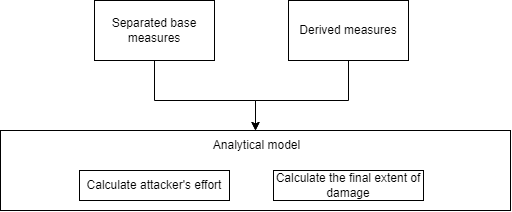
\includegraphics[width=10cm]{pictures/impl_ana_mod.png}
  \caption{The analytical model takes the separated base measures and derived measures. Then it distribute them to the inner analytical models.}
  \label{fig:impl_ana_mod}
\end{figure}

The last step to get the measurement results shows Figure \ref{fig:impl_dec_criteria} which input for the decision criteria are the two possible indicators from Figure \ref{fig:impl_ana_mod}. The attacker's effort have to be in an interval which have to be specified as an information need. The extent of damage must also be checked based on an information need \cite{ISO_27004_2009}. For this thesis there is no interval because the information need is not considered further. If the criteria is fulfilled the indicatos are able to be calculated and then the result can be depicted. This procedure describe subsection \ref{sec:impl_meas_res}.

\begin{figure}[ht!]
  \centering
  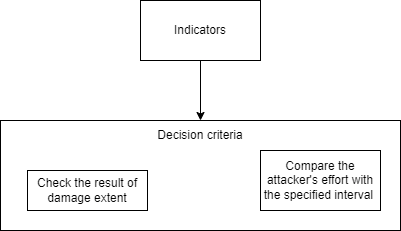
\includegraphics[width=10cm]{pictures/impl_dec_criteria.png}
  \caption{The analytical model takes the separated base measures and derived measures. Then it distribute them to the inner analytical models.}
  \label{fig:impl_dec_criteria}
\end{figure}

\subsection{Evaluation Method}

The following steps describe the complete process on how the $Risk$ can be depicted in the risk matrix (the flow graph depict in Figure \ref{fig:flow_graph} the process of this evaluation) \cite{DBLP:journals/corr/abs-2012-04884}:

\begin{enumerate}
  \item All weights are chosen based on result's impact of each risk indicator on a ML model.
  \item Each value of a risk indicator is assigned to a weight which represent the impact on the extent of damage or probability of occurrence.
  \item The value of a risk indicator is mapped with the identified weights.
  \item The weights depict the structure of the risk matrix.
  \item Then the calculated $Risk$ is depict in the risk matrix.
\end{enumerate}

\begin{figure}[h!]
  \centering
  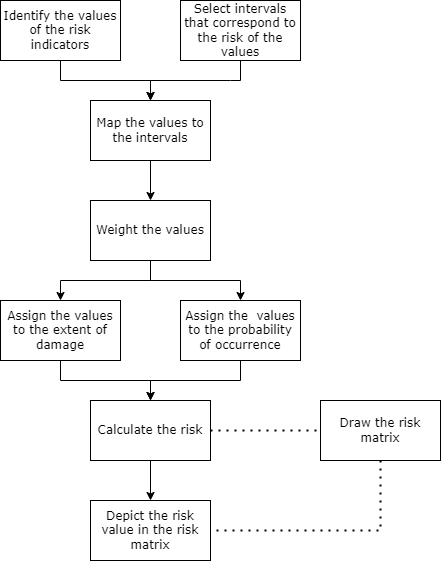
\includegraphics[width=10cm]{pictures/flow_graph.png}
  \caption{The process to depict the $Risk$ on the risk matrix.}
  \label{fig:flow_graph}
\end{figure}

The goal of this flow graph is to weight the $Risk$ based on the original ML model. For example, if the accuracy is $90\%$ then this value represents the best approximation for the $Risk$ value in the risk matrix. The same weighting applies for the other risk indicators which are able to differentiate between the original and attacked ML model. This weighting could make it possible for an organization to decide the lowest and highest $Risk$ based on the output data and to create the decision criteria.

\subsection{Show the measurement results}
\label{sec:impl_meas_res}

The measurement results show the monitored data based on the measurement process of ISO 27004 \cite{ISO_27004_2009}. This contains all logged risk indicator values and visualized ML metrics. A second part shows the risk for the ML model with an attack. The risk is calculated by $Risk = $ \textit{Extent of damage} $*$ \textit{Probability of occurence} \cite{DBLP:journals/access/JianxingHSH21}. This risk value is depicted in a risk matrix which shows how high the risk is with the executed attack. Based on the measurement result should it be possible to interpret the attack but the RMF shows no defense methods. The RMF concentrates only on the attack and the associated risk measurement. What happens with these results and what they are used for remains open. The following section evaluates the RMF risk measurement based on a case study which contains the street sign classification on autonomous driving which is attacked by different backdoor attacks separately.

\subsection{The logging function}

To show all steps of the risk measurement the RMF has a function that documents them. Assigned values of the risk indicators, the pre-determined steps to measure the attacker's effort, and the calculations of the risk measurement are represented with an optimized logging function, based on the Python logging module. The function takes two arguments such as a message string and the wanted logging level (i.e. INFO or DEBUG). The following example shows an execution of the logging function:

\begin{lstlisting}
  log(f"{variable_name}", 'INFO')
\end{lstlisting}

This function should make it possible for human judgment to find the critical parts where the ML model is particularly vulnerable for backdoor attacks. The next section evaluates the implemented concept from this section and present the results of a case study which uses the RMF to measure risks of a ML model backdoor attack.
